
%% bare_jrnl_compsoc.tex
%% V1.4b
%% 2015/08/26
%% by Michael Shell
%% See:
%% http://www.michaelshell.org/
%% for current contact information.
%%
%% This is a skeleton file demonstrating the use of IEEEtran.cls
%% (requires IEEEtran.cls version 1.8b or later) with an IEEE
%% Computer Society journal paper.
%%
%% Support sites:
%% http://www.michaelshell.org/tex/ieeetran/
%% http://www.ctan.org/pkg/ieeetran
%% and
%% http://www.ieee.org/

%%*************************************************************************
%% Legal Notice:
%% This code is offered as-is without any warranty either expressed or
%% implied; without even the implied warranty of MERCHANTABILITY or
%% FITNESS FOR A PARTICULAR PURPOSE! 
%% User assumes all risk.
%% In no event shall the IEEE or any contributor to this code be liable for
%% any damages or losses, including, but not limited to, incidental,
%% consequential, or any other damages, resulting from the use or misuse
%% of any information contained here.
%%
%% All comments are the opinions of their respective authors and are not
%% necessarily endorsed by the IEEE.
%%
%% This work is distributed under the LaTeX Project Public License (LPPL)
%% ( http://www.latex-project.org/ ) version 1.3, and may be freely used,
%% distributed and modified. A copy of the LPPL, version 1.3, is included
%% in the base LaTeX documentation of all distributions of LaTeX released
%% 2003/12/01 or later.
%% Retain all contribution notices and credits.
%% ** Modified files should be clearly indicated as such, including  **
%% ** renaming them and changing author support contact information. **
%%*************************************************************************


% *** Authors should verify (and, if needed, correct) their LaTeX system  ***
% *** with the testflow diagnostic prior to trusting their LaTeX platform ***
% *** with production work. The IEEE's font choices and paper sizes can   ***
% *** trigger bugs that do not appear when using other class files.       ***                          ***
% The testflow support page is at:
% http://www.michaelshell.org/tex/testflow/


\documentclass[10pt,journal,compsoc]{IEEEtran}
%
% If IEEEtran.cls has not been installed into the LaTeX system files,
% manually specify the path to it like:
% \documentclass[10pt,journal,compsoc]{../sty/IEEEtran}


\usepackage[T1]{fontenc}
\usepackage[utf8]{inputenc}
\usepackage[ngerman]{babel}

%% asm
\usepackage{amsmath}
\usepackage{amsfonts}
\usepackage{amssymb}

%% utilities
\usepackage{graphicx}
\usepackage{tikz}
\usepackage{multicol}
\usepackage{slashbox}
\usepackage{ntheorem}
\usepackage{listings}
\usepackage{color}

\definecolor{mygreen}{rgb}{0,0.6,0}
\definecolor{mygray}{rgb}{0.5,0.5,0.5}
\definecolor{mymauve}{rgb}{0.58,0,0.82}

\lstset{ %
  backgroundcolor=\color{white},   % choose the background color; you must add \usepackage{color} or \usepackage{xcolor}; should come as last argument
  basicstyle=\footnotesize,        % the size of the fonts that are used for the code
  breakatwhitespace=false,         % sets if automatic breaks should only happen at whitespace
  breaklines=true,                 % sets automatic line breaking
  captionpos=b,                    % sets the caption-position to bottom
  commentstyle=\color{mygreen},    % comment style
  deletekeywords={...},            % if you want to delete keywords from the given language
  escapeinside={(*}{*)},          % if you want to add LaTeX within your code
  extendedchars=true,              % lets you use non-ASCII characters; for 8-bits encodings only, does not work with UTF-8
  frame=single,	                   % adds a frame around the code
  keepspaces=true,                 % keeps spaces in text, useful for keeping indentation of code (possibly needs columns=flexible)
  keywordstyle=\color{blue},       % keyword style
  language=Python,                 % the language of the code
  morekeywords={*,...},           % if you want to add more keywords to the set
  numbers=left,                    % where to put the line-numbers; possible values are (none, left, right)
  numbersep=8pt,                   % how far the line-numbers are from the code
  numberstyle=\tiny\color{mygray}, % the style that is used for the line-numbers
  rulecolor=\color{black},         % if not set, the frame-color may be changed on line-breaks within not-black text (e.g. comments (green here))
  showspaces=false,                % show spaces everywhere adding particular underscores; it overrides 'showstringspaces'
  showstringspaces=false,          % underline spaces within strings only
  showtabs=false,                  % show tabs within strings adding particular underscores
  stepnumber=1,                    % the step between two line-numbers. If it's 1, each line will be numbered
  stringstyle=\color{mymauve},     % string literal style
  tabsize=2,	                   % sets default tabsize to 2 spaces
  title=\lstname                   % show the filename of files included with \lstinputlisting; also try caption instead of title
}

% *** CITATION PACKAGES ***
%
\ifCLASSOPTIONcompsoc
  % IEEE Computer Society needs nocompress option
  % requires cite.sty v4.0 or later (November 2003)
  \usepackage[nocompress]{cite}
\else
  % normal IEEE
  \usepackage{cite}
\fi
% *** GRAPHICS RELATED PACKAGES ***
%
\ifCLASSINFOpdf
  % \usepackage[pdftex]{graphicx}
  % declare the path(s) where your graphic files are
  % \graphicspath{{../pdf/}{../jpeg/}}
  % and their extensions so you won't have to specify these with
  % every instance of \includegraphics
  % \DeclareGraphicsExtensions{.pdf,.jpeg,.png}
\else
  % or other class option (dvipsone, dvipdf, if not using dvips). graphicx
  % will default to the driver specified in the system graphics.cfg if no
  % driver is specified.
  % \usepackage[dvips]{graphicx}
  % declare the path(s) where your graphic files are
  % \graphicspath{{../eps/}}
  % and their extensions so you won't have to specify these with
  % every instance of \includegraphics
  % \DeclareGraphicsExtensions{.eps}
\fi

% *** PDF, URL AND HYPERLINK PACKAGES ***
%
\usepackage{url}
% url.sty was written by Donald Arseneau. It provides better support for
% handling and breaking URLs. url.sty is already installed on most LaTeX
% systems. The latest version and documentation can be obtained at:
% http://www.ctan.org/pkg/url
% Basically, \url{my_url_here}.

% correct bad hyphenation here
\hyphenation{op-tical net-works semi-conduc-tor}


\begin{document}
%
% paper title
% Titles are generally capitalized except for words such as a, an, and, as,
% at, but, by, for, in, nor, of, on, or, the, to and up, which are usually
% not capitalized unless they are the first or last word of the title.
% Linebreaks \\ can be used within to get better formatting as desired.
% Do not put math or special symbols in the title.
\title{Concolutional Neural Network for classification of handwritten digits}
\markboth{Machine Learning - Deep Learning,~Project 1}%
{}

% for Computer Society papers, we must declare the abstract and index terms
% PRIOR to the title within the \IEEEtitleabstractindextext IEEEtran
% command as these need to go into the title area created by \maketitle.
% As a general rule, do not put math, special symbols or citations
% in the abstract or keywords.
\IEEEtitleabstractindextext{%
\begin{abstract}
In diesem Projekt haben wir ein \emph{convolutional neural network} zur Klassifikation von handgeschriebenen Ziffern implementiert. Wir haben zwei \emph{convolutional} Schichten, gefolgt von zwei \emph{fully-connected} Schichten in unserer Architektur umgesetzt. Nach jeder Faltung addieren wir ein \emph{bias} und wenden dann als Aktivierung die \emph{ReLU} an. Dann wird jeweils \emph{max-pooling} dahinter geschaltet um die Anzahl der Parameter zu reduzieren, ohne den Verlust der wesentlichen Merkmale. Auch bei den \emph{fully-connected} Schichten kommt \emph{ReLU} zum Einsatz und zum Schluss benutzen wir \emph{softmax} um auf die zehn Klassen ein \emph{scope} auszugeben. Trainiert und getestet wurde mit dem MNIST Datensatz, dabei diente TensorFlow als Framework zur Modellierung des Netzes der in Python implementiert wird. Wir haben uns auf einige wesentliche Fragestellungen bezüglich der Architektur konzentriert, um am Ende der Analyse dieser Fragen, eine möglichst
gute CNN Architektur zur Klassifikation von handgeschriebenen Ziffern zu erhalten.
\end{abstract}

% Note that keywords are not normally used for peerreview papers.
\begin{IEEEkeywords}
Machine Learning, Deep Learning, CNN, Neural Network, MNIST, handwritten digits
\end{IEEEkeywords}}

% make the title area
\maketitle
\IEEEdisplaynontitleabstractindextext
\IEEEpeerreviewmaketitle
\IEEEraisesectionheading{\section{Einleitung}\label{sec:introduction}}
\IEEEPARstart{I}{m} Rahmen des ersten praktischen Projekts der Vorlesung \glqq Machine Learning II - Deep Learning\grqq\ haben wir ein Convolutional Neural Network, kurz CNN, selbst programmiert und umfangreich getestet. Als Trainings- und Testdatensatz nutzen wir dazu den bereits vom verwendeten Framework \glqq Tensorflow\grqq\ mitgelieferten MNIST Datensatz \glqq Handwritten Digits\grqq\. Durch Einsatz verschiedener Kombinationen von convolutional layers und pooling layers konnten wir die darin enthaltenen handschriftlich notierten Zahlen klassifizieren. Die Fehlerrate konnten wir durch den Einsatz von zwei convolutional layers und zwei pooling layers mit einer learning rate von 0.01 bzw. einer adaptive Rate bis auf 2\% beschränken.

\section{Die Architektur}
Unsere Architektur besteht insgesamt aus sechs Layern.
Dabei ist unsere Architektur in einen Teil von Convolutional und Pooling Layern und einen Teil Fully Connected Layer unterteilt. Unsere beiden Convulutional Layer haben jeweils ReLU als Aktivierungsfunktion und einen nachgestellten Pooling Layer zur Reduzierung der Datenmenge. Auf dieser Layer folgen zwei Fully Connected Layer, wobei zwischen den Layern noch Dropout verwendet wird.\\

\noindent Nun zu der Entstehung unserer Architektur. Wir haben unser neuronales Netz ausgehend von der vorherigen Übung aufgebaut, dabei haben wir schrittweise mehr Layer hinzugefügt und die Funktionalität unseres Netzes nach jedem Schritt überprüft. Zuerst haben wir einen Convulutional Layer samt Aktivierungsfunktion eingefügt. Daraufhin haben wir, wie es in der Vorlesung schon beschrieben wurde, einen Pooling Layer hinter die Convulution geschaltet. Dies haben wir wiederholt und einen zweiten Convulutional Layer samt Aktivierung und Pooling eingefügt. Diesmal mit einer anderen Filtergröße. Um unsere Ergebnisse weiter zu verbessern, haben wir einen zweiten Fully Connected Layer vor den Ausgabelayer geschaltet. Außerdem kam als letztes noch Dropout zwischen den beiden Fully Connected Layern als Funktion dazu.\\

\noindent Unsere Convulutional Layer nutzten in unseren Versuchen Filter in den Größen zwischen $3\times 3$ und $7\times 7$, wobei wir in unserer finalen Konfiguration nicht über eine Filtergröße hinausgehen. Außerdem haben wir in den Layern mit der Anzahl der Filter zwischen 16 und 64 experimentiert, wobei bereits mit 16 Filtern eine Genauigkeit von über 90\% erzielt wurde.\\

\noindent Als Pooling nutzen wir $2\times 2$-max-Pooling mit 2er Strides zur Reduzierung der Auflösung der Inputdaten. Damit brechen wir die Daten insgesamt von $28\times 28$ Pixel auf $7\times 7$-Pixel herunter. Dies wirkt sich enorm positiv auf die Laufzeit unseres Netzes aus. Eine weitere Reduzierung der Auflösung war uns jedoch nicht möglich, da 7 prim ist.\\

\noindent Bei unserem extra Fully Connected Layer haben wir mit der Anzahl der Neuronen bei 50 begonnen und sind bis 128 hochgegangen.

Die \emph{keep probability} bei unserem \emph{Dropout} haben wir zwischen 50\% und 90\% schwanken lassen, ohne dass sich Auswirkungen auf das Ergebnis gezeigt hätten.
Generell war unsere Architektur maßgeblich durch den verfügbaren Arbeitsspeicher der Hardware begrenzt. Bei Versuchen mit mehr Convulution Filtern oder einer höheren Anzahl an Neuronen in den Fully Connected Layern traten sehr schnell Speicherfehler auf, welche zum Absturz unseres Netzes führten.\\

\newpage
\noindent Nun noch einmal unsere Architektur in Kurzform:

\begin{scriptsize}
\textbf{
C(32, 5, 1)-ReLU-P(2, 2)-C(64, 3, 1)-ReLU-P(2, 2)-F(128)-D(.9)-F(10)}
\end{scriptsize}

\begin{itemize}
\item[-] $C(X, Y, Z)$ ~ Convulution mit $X$ Filtern, $Y$ quadratischer Filtergröße, $Z$ Stride
\item[-] ReLU ~ Rectified Linear Unit
\item[-] $P(X, Y)$ ~ Pooling mit $X$ quadratischem Filter und $Y$ Stride
\item[-] $F(X)$ ~ Fully Connected mit $X$ Neuronen
\item[-] $D(X)$ ~ Dropout mit keep probability $X$
\end{itemize}

\section{Das Training}

In einem Versuch haben wir die beiden von uns verwendeten Max-Pooling-Layer entfernt.
Da wir in unseren Convolutional Layern stets Stride 1 verwenden, führt das Entfernen der Pooling-Layer natürlich dazu, dass das gesamte Netzwerk zunächst die Inputgröße beibehält.\\

\noindent Dadurch vergrößert sich die Trainingszeit bedeutend. In unserem Fall haben wir im Schnitt einen zeitlichen Mehraufwand von Faktor 2 bis 3 gemessen.
Die Accuracy veränderte sich dabei nicht bedeutend. In den meisten Fällen war sogar eine Verschlechterung der Accuracy zu verzeichnen.\\

\begin{figure}[!h]
\centering
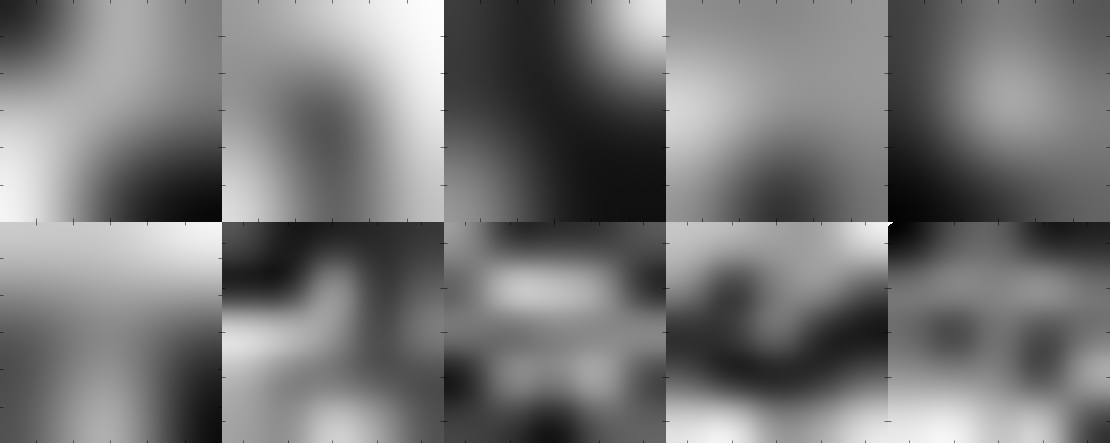
\includegraphics[scale=0.25]{learned_conv_filter_from_first_and_second_layer}
\caption{Gelernte Filter aus der ersten und zweiten Faltungs-Schicht.}
\end{figure}

\noindent Im folgenden werden unsere Ergebnisse mit unterschiedlichen Learning Rates beschrieben, dabei wurde der AdamOptimizer genutzt.
Die zufällige Initialisierung unseres Netzes erreichte in der ersten Runde des Trainings immer eine ungefähre Trefferrate von 10\%.
Die schlechtesten Ergebnisse erhielten wir mit einer Learning Rate von 1. Dabei hat das Netz durch Training keinerlei Verbesserung erfahren und erzielte weiterhin Klassifizierungsraten von circa 10\%.\\

\noindent Daraufhin haben wir die Learning Rate im nächsten Schritt auf 0.5 verringert. Auf die Qualität des Netzes hatte dies keinen Einfluss - die Ergebnisse waren genauso schlecht wie vorher.
Auch bei einer Learning Rate von 0.1 erzielten wir eine Klassifikationsrate von 0.1.
Die besten Ergebnisse lieferte uns jedoch eine Learning Rate 0.01 bzw. eine nicht-eingestellte Learning Rate, die vom Netz selbst angepasst wird. Dabei erreichten wir eine Genauigkeit von 98\% auf den Testdaten.

\section{Test und Auswertung}
Wir haben beobachtet, dass die Test-Accuracy am Anfang relativ schnell auf über 90\% steigt und dann gegen einen Wert, nahe bei 100\% strebt. Besonders mit einer festen Learningrate stellt man Schwankungen in der Training-Accuracy fest, dies wird bei adaptiver Leraning-Rate und bei beobachtung der Test-Accuracy deutlich stabiler.
\begin{figure}[!h]
\centering
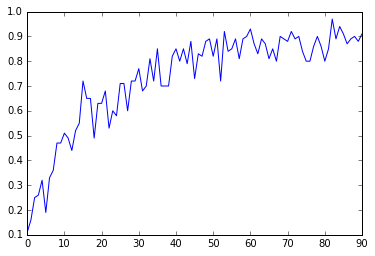
\includegraphics[scale=0.5]{accuracy_90_iterations_fixed_learning_rate}
\caption{Training \emph{accuracy} mit konstanter Lernrate in 90 iterationen, Batch-Größe 100.}
\end{figure}

Um eine Test-Accuracy von über 98\% zu erreichen, benötigt ein Rechner (z.B. aktueller Laptop) eine Rechenzeit von einigen wenigen Minuten. Die Trainingsdaten werden gut generalisiert, sodass keine zusätzliche \emph{overfitting}-Prevention nötig ist. Bei gleicher Konfiguration bekommt man dennoch leicht unterschiedliche Ergebnisse, weil die Initialisierung zufällig ist. Dennoch kann man insgesamt ein konvergentes Verhalten beobachten.

\begin{figure}[!h]
\centering
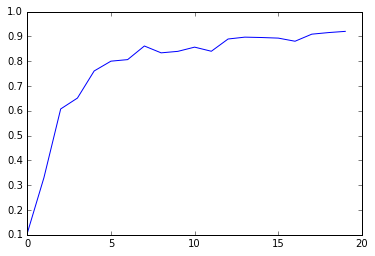
\includegraphics[scale=0.5]{test_accuracy_adapt_rate}
\caption{Test \emph{accuracy} bei adaptiver Lernrate.}
\end{figure}
\appendices
\section{Code-Schnipsel}

\begin{lstlisting}[caption={Erzeugt ein Gewichts-Array mit zufällig initialisierten Werten. Die Dimensionen werden als Parameter entegengenommen.}, label=lst1]
def weight_variable(shape):
    """Creates a tf Variable of shape 'shape' with random elements"""
    initial = tf.truncated_normal(shape, stddev=0.1)
    return tf.Variable(initial)
\end{lstlisting}

\begin{lstlisting}[caption={Erzeugt ein bias-Array mit zufällig initialisierten Werten. Die Dimensionen werden als Parameter entegengenommen.}, label=lst2]
def bias_variable(shape):
    """Create a small bias of shape 'shape' with contants values of 0.1"""
    initial = tf.constant(0.1, shape=shape)
    return tf.Variable(initial)
\end{lstlisting}

\begin{lstlisting}[caption={Eine zweidimensionale Faltung mit Eingabe x und Filter W.}, label=lst3]
def conv2d(x, W):
    """Use a conv layer with weights W on zero padded input x and stride 1"""
    return tf.nn.conv2d(x, W, strides=[1, 1, 1, 1], padding='SAME')
\end{lstlisting}

\begin{lstlisting}[caption={Hier wird 2x2 max pooling auf die Eingabe x angewendet.}, label=lst4]
def max_pool_2x2(x):
    """Create a 2x2 pooling layer with strides 2, reducing the resolution"""
    return tf.nn.max_pool(x, ksize=[1, 2, 2, 1], strides=[1, 2, 2, 1], padding='SAME')
\end{lstlisting}

\begin{lstlisting}[caption={Modellierung des Berechnungsgraphen.}, label=lst5]
# x is 1x28*28 ( x = [34,43,5,6,0,0,7,5,...] )
# W_conv1 is 5x5
# b_conv1 is 1x32
W_conv1 = weight_variable([5,5,1,32])
b_conv1 = bias_variable([32])
# input data is embedded in 4d tensor
x_image = tf.reshape(x, [-1, 28, 28, 1])
# h_conv1 is result of applied conv filter W to x
h_conv1 = tf.nn.relu(conv2d(x_image, W_conv1) + b_conv1)
h_pool1 = max_pool_2x2(h_conv1)

# Apply second convolutional layer
W_conv2 = weight_variable([3, 3, 32, 64])
b_conv2 = bias_variable([64])
h_conv2 = tf.nn.relu(conv2d(h_pool1, W_conv2) + b_conv2)
    
h_pool2 = max_pool_2x2(h_conv2)

#Fully connected layer
W_fc1 = weight_variable([7 * 7 * 64, 128])
b_fc1 = bias_variable([128])
h_pool2_flat = tf.reshape(h_pool2, [-1, 7*7*64])
h_fc1 = tf.nn.relu(tf.matmul(h_pool2_flat, W_fc1) + b_fc1)

keep_prob = tf.placeholder(tf.float32)
h_fc1_drop = tf.nn.dropout(h_fc1, keep_prob)

W_fc2 = weight_variable([128, MNIST_CLASSES])
b_fc2 = bias_variable([MNIST_CLASSES])

y_conv = tf.matmul(h_fc1_drop, W_fc2) + b_fc2
\end{lstlisting}

% Can use something like this to put references on a page
% by themselves when using endfloat and the captionsoff option.
\ifCLASSOPTIONcaptionsoff
  \newpage
\fi

\begin{thebibliography}{1}
\bibitem{vorlesung}
TODO: Namen einfügen, \emph{Vorlesung: Machine Learning II - Deep Learning}, WS 2016/17
\end{thebibliography}
\end{document}


